%%%% PROCESAR con PdfLaTeX !!!!!


\documentclass[12pt]{book}
\usepackage[T1]{fontenc}
\usepackage{lmodern}
\usepackage{geometry}\geometry{top=2cm,bottom=2cm,left=2cm,right=2cm}
\usepackage{amssymb}
\usepackage{amsmath}
\usepackage{graphicx}
%\usepackage{txfonts}
%\usepackage{hyperref}
\usepackage[hidelinks]{hyperref}
\usepackage[spanish]{babel}
\setcounter{tocdepth}{4}
\usepackage[usenames]{color}
\usepackage{pdfpages}
\usepackage{enumerate}
\usepackage{framed}
\usepackage{color}
\usepackage{wrapfig}\definecolor{shadecolor}{RGB}{224,238,238}


\usepackage{multirow, array} % para las tablas
\usepackage{float} % para usar [H]




\usepackage[hidelinks]{hyperref}
\hypersetup{
    colorlinks=true,
    linkcolor=blue,
    filecolor=magenta,      
    urlcolor=cyan,
    pdftitle={Sharelatex Example},
    bookmarks=true,
%    pdfpagemode=FullScreen,
}



\begin{document}
\thispagestyle{empty}

\begin {center}


\includegraphics[scale=.4]{./img/logo.jpeg}


\medskip
\textbf{\large UNIVERSIDAD DE BUENOS AIRES}

Facultad de Ciencias Económicas \\
Departamento de Economía

\vspace{3cm}



\textbf{\large MICROECONOMIA I}

\vspace{2cm}


Este es un modesto aporte para los alumnos de la f\'acultad de Econom\'ia  de la UBA.
De ninguna man\'era pretende ser una gu\'ia de estudio, ni remplaza las clases presenciales, el material oficial de la catedra esta disponible en el web site de la m\'ateria.
\\
\end {center}


\vspace{2.5cm}

\noindent Autor:	\,Isaac Edgar Camacho Ocampo
 
\noindent Carrera:	\,Licenciatura en Economía


\vspace{1cm}

\vspace{1cm}

\noindent Buenos Aires, 2025
\vspace{1cm}
\\
\textit{Si se encuentra alg\'un error u omisi\'on en este res\'umen por favor colaborar en  \\
\url{https://github.com/IsaacEdgarCamacho/Apuntes/} \quad \\ o escribirme a 
\url{isaac.edgar.camacho@gmail.com}
}
\newpage


\tableofcontents



\chapter{Economía}
%Es el estudio de la manera en que la sociedad decide emplear los recursos productivos escasos que pueden utilizarse con distintos fines, producir mercaderías y distribuirlas. 	
%La economía es una ciencia porque trata de interpretar los fenómenos del mundo real mediante el empleo de un procedimiento riguroso y apropiado. Está incluida dentro de las Ciencias Sociales. 
%
%\section{Microeconomía:} es la rama de la economía que se ocupa de la conducta de entidades individuales como los mercados, las empresas y los hogares.  	
%\section{Macroeconomía:} rama que se ocupa del funcionamiento general de la Economía. 	
% 	


%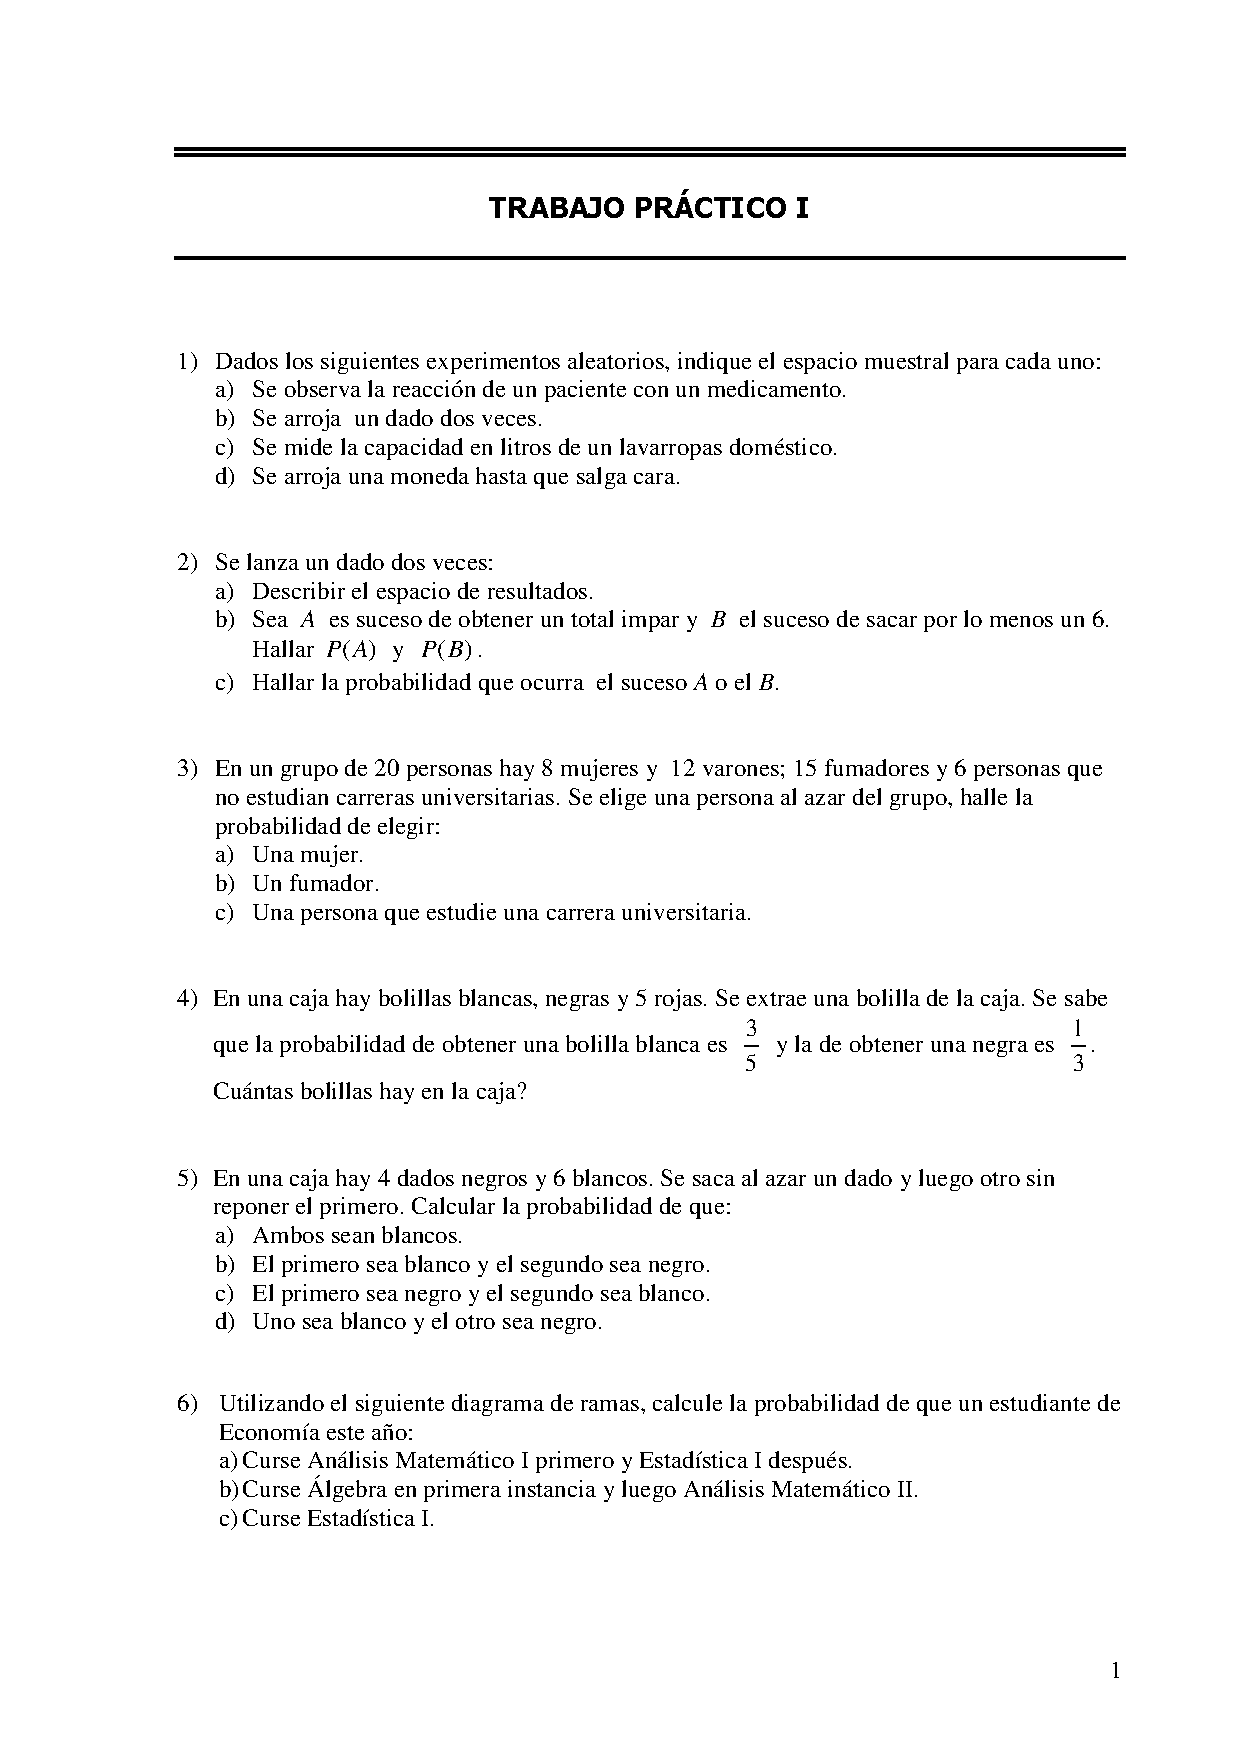
\includepdf[pages=-]{./pdfs/p1.pdf}
\section{Prácita 1}
\begin{center}
    
\includegraphics[scale=.8]{./img/p1/ej1.png}    
\end{center}


\begin{enumerate}[a)]
\item La idéa es pensar en 3 posiciones y cada una tiene 3 resultados posibles.\\ 3 . 3 . 3 = $3^3$ = 27
\item Ahora son 37 posiciones y cada una tiene 3 resultados posibles. \\
3 . 3 . 3 ... 3 = $ 3^{37} $ = 450283905890997363 = $ 4,5028391. 10^{17} $ 
\item generalizando, tenemos $ r.r.r.....r = r^n$
\end{enumerate}

\end{document}


